% Entrega 1: Diseño del esquema NoSQL y plan de implementación
% Compilar desde docs/delivery1/:  latexmk -pdf entrega1.tex
\documentclass[11pt,a4paper]{article}

\usepackage[T1]{fontenc}
\usepackage[utf8]{inputenc}
\usepackage[spanish,es-noshorthands,es-tabla]{babel}
\usepackage{lmodern}
\usepackage[left=2.3cm,right=2.3cm,top=2.2cm,bottom=2.4cm]{geometry}
\usepackage{graphicx}
\usepackage{booktabs}
\usepackage{float}
\usepackage{tabularx}
\usepackage{array}
\usepackage{xcolor}
\usepackage{enumitem}
\usepackage[font=small,labelfont=bf]{caption}
\usepackage{fancyhdr}
\usepackage[hidelinks]{hyperref}

\definecolor{acento}{HTML}{1F5FAF}
\newcommand{\brkus}{\textunderscore\allowbreak}
\newcommand{\f}[1]{{\ttfamily\let\_\brkus #1}}
\hyphenation{MUNICIPALITY BUILDING ROOFTOP INGESTION SUBREGION DATASET}
\newcolumntype{L}{>{\raggedright\arraybackslash}X}
\setlist{nosep,leftmargin=1.4em}
\setlength{\parskip}{0.45em}
\setlength{\parindent}{0pt}
\renewcommand{\arraystretch}{1.15}

\pagestyle{fancy}
\fancyhf{}
\lhead{\small Proyecto final DBA · Entrega 1}
\rhead{\small Techos solares en municipios PDET}
\cfoot{\small \thepage}
\renewcommand{\headrulewidth}{0.3pt}

\begin{document}

\begin{center}
  {\small Pontificia Universidad Javeriana · Administración de Bases de Datos · 2026-30}\\[0.9em]
  {\LARGE\bfseries\color{acento} Entrega 1: Diseño del esquema NoSQL\\[0.2em] y plan de implementación}\\[0.8em]
  {\large Potencial solar en techos de los municipios PDET (UPME)}\\[0.8em]
  Derek Sarmiento · José Medina · Miguel Duarte · Sebastián Sánchez Vásquez · Samuel Emperador\\[0.3em]
  {\small Prof. Andrés Oswaldo Calderón Romero, Ph.D. · Lunes 2 de noviembre de 2026}\\[0.3em]
  {\small Repositorio: \url{https://github.com/dba-upme-pdet/techos-solares-pdet}}
\end{center}

\section{Objetivo y alcance}

La UPME necesita ordenar los 170 municipios PDET según el área de techos disponible para paneles solares. Para cada municipio vamos a calcular cuántas edificaciones tiene y cuánta área de techo suman, con dos fuentes abiertas de huellas de edificaciones (Microsoft Building Footprints y Google Open Buildings v3) y MongoDB como motor NoSQL. El ranking final ordena los municipios por \f{total\_area\_m2} y se presenta por separado para cada fuente.

Esta entrega define la metodología y el modelo de datos sobre los que se construyen las entregas 2 a 5: (a) plan de implementación, (b) diagrama E-R y (c) diccionario de datos. Todavía no se cargan datos; el esquema ya se puede crear con \f{scripts/00\_init\_db.py} (sección~\ref{sec:indices}).

\section{Decisiones tecnológicas}

\subsection{Motor NoSQL: MongoDB 7}

MongoDB guarda geometrías como GeoJSON, las indexa con \f{2dsphere} y resuelve punto en polígono con \f{\$geoWithin}. El conteo y la suma por municipio se hacen en su pipeline de agregación, sin sacar los datos de la base. Corre en Docker (\f{docker-compose.yml}).

\begin{table}[H]
\centering\small
\caption{Motores NoSQL evaluados.}
\begin{tabularx}{\textwidth}{@{}l L l L p{3.1cm}@{}}
\toprule
Motor & Tipos geográficos & Índice & Agregación por polígono & Decisión \\
\midrule
MongoDB & Point, Polygon, MultiPolygon (GeoJSON) & 2dsphere & \f{\$geoWithin} + \f{\$group} & Elegido \\
Elasticsearch & geo\_point, geo\_shape & Árbol BKD & geo\_shape + agregaciones & Respaldo; exige más memoria y configuración \\
Cassandra & Ninguno (requiere GeoMesa) & Externo & Débil & Descartado \\
Neo4j & Solo puntos & De puntos & No admite polígonos & Descartado \\
\bottomrule
\end{tabularx}
\end{table}

MongoDB no calcula áreas geodésicas. El área de cada huella se calcula en Python (\f{pyproj.Geod}) durante la carga y se guarda como campo.

\subsection{Fuentes de datos}

\begin{table}[H]
\centering\small
\caption{Fuentes seleccionadas. Las dos de edificaciones entregan polígonos 2D para toda Colombia, así que se cuentan y miden con el mismo método.}
\begin{tabularx}{\textwidth}{@{}p{3.3cm} L L p{1.4cm}@{}}
\toprule
Fuente & Formato & Atributos clave & Rol \\
\midrule
Microsoft Building Footprints (ODbL) & GeoJSON Lines por quadkey; índice \f{dataset-links.csv} & polígono, \f{confidence}, \f{height} ($-1$ si no se conoce) & Fuente A \\
Google Open Buildings v3 (CC BY-4.0 / ODbL) & CSV.gz por celda S2 & polígono WKT, \f{area\_in\_meters}, \f{confidence}, \f{full\_plus\_code} & Fuente B \\
GlobalBuildingAtlas (TUM) & Teselas 3D LoD1 & polígono + altura (3D); el proyecto solo necesita la huella 2D & No se usa \\
DANE MGN 2025, nivel municipal & Shapefile en ZIP (1,5 GB), EPSG:4686 & \f{MPIO\_CDPMP}, \f{MPIO\_CNMBR}, \f{MPIO\_NAREA} & Límites \\
\f{MunicipiosPDET.xlsx} (curso) & Excel, 170 filas & subregión, código DANE & Filtro PDET \\
\bottomrule
\end{tabularx}
\end{table}

El MGN y la lista PDET se cruzan por el código DIVIPOLA de 5 dígitos, nunca por nombre. El campo \f{area\_in\_meters} de Google sirve para validar el área que calculamos.

\section{Plan de implementación}

Cada paso es un script numerado en \f{scripts/} que lee rutas, URLs y umbrales de \f{config.yaml}, para correr el flujo de principio a fin sin pasos manuales.

\begin{table}[H]
\centering\small
\caption{Fases del flujo, una por entrega.}
\begin{tabularx}{\textwidth}{@{}>{\raggedright\arraybackslash}p{2.3cm} L >{\raggedright\arraybackslash}p{4.3cm}@{}}
\toprule
Fase (entrega) & Pasos & Scripts y salida \\
\midrule
0. Entorno (E1) &
MongoDB 7 en Docker; Python 3.11 con \f{pymongo}, \f{geopandas}, \f{shapely}, \f{pyproj}; crear colecciones, validadores e índices. Verificar la lista PDET: 170 municipios, 16 subregiones. &
\f{00\_check\_environment.py}\newline \f{00\_check\_pdet\_list.py}\newline \f{00\_init\_db.py} \\
\addlinespace
1. Límites PDET (E2) &
Descargar el MGN 2025 y extraer la capa municipal. Rellenar los códigos del Excel a 5 dígitos (5031 $\rightarrow$ 05031), cruzar y registrar los que no crucen. Reproyectar de EPSG:4686 a EPSG:4326, reparar geometrías con \f{make\_valid}, revisar el límite de 16 MB por documento. &
\f{01\_download\_mgn.py}\newline \f{02\_load\_municipalities.py}\newline $\rightarrow$ \f{municipalities} \\
\addlinespace
2. Huellas (E3) &
Descargar solo las particiones (quadkey, celda S2) que tocan los rectángulos envolventes PDET. Leer por bloques y descartar lo que cae fuera. Por edificación: validar polígono, calcular área geodésica y centroide. \f{insert\_many} no ordenado en lotes de 10\,000; índices después de la carga. EDA. &
\f{03\_download\_buildings.py}\newline \f{04\_load\_buildings.py}\newline \f{05\_eda.ipynb}\newline $\rightarrow$ \f{buildings}, \f{ingestion\_runs} \\
\addlinespace
3. Conteo y área (E4) &
Asignar cada edificación al municipio que contiene su centroide (\f{\$geoWithin}); aplicar confianza y área mínimas; \f{\$group} por municipio y fuente. Exportar tablas CSV y mapas coropléticos. &
\f{06\_rooftop\_stats.py}\newline \f{07\_maps.ipynb}\newline $\rightarrow$ \f{rooftop\_stats}, \f{outputs/} \\
\addlinespace
4. Informe (E5) &
Metodología, resultados, comparación de fuentes, ranking de municipios y recomendaciones para la UPME. &
\f{docs/delivery5/} \\
\bottomrule
\end{tabularx}
\end{table}

\textbf{Bordes municipales.} Asignar por centroide pone cada edificación en un solo municipio, así que una edificación sobre un límite no se cuenta dos veces. La fase 3 solo llena \f{mpio\_code} si sigue vacío, de modo que un centroide justo sobre un borde compartido queda en el primer municipio procesado. Si el centroide no cae en ningún municipio PDET, \f{mpio\_code} queda en \f{null} y la edificación no entra en el conteo.

\textbf{Umbrales pendientes.} Área mínima (candidato: 20\,m\textsuperscript{2}) y confianza mínima (candidato: 0,70 para Google; el campo de Microsoft suele venir vacío). Se fijan con el EDA de la Entrega 3. El área de huella es un límite superior del área útil para paneles: no descuenta orientación, sombra ni pendiente. El informe final lo discute.

\section{Modelo de datos}

Seis entidades, cada una guardada como una colección. \f{BUILDING} es la entidad central y la de mayor volumen (millones de documentos).

\begin{figure}[htbp]
\centering
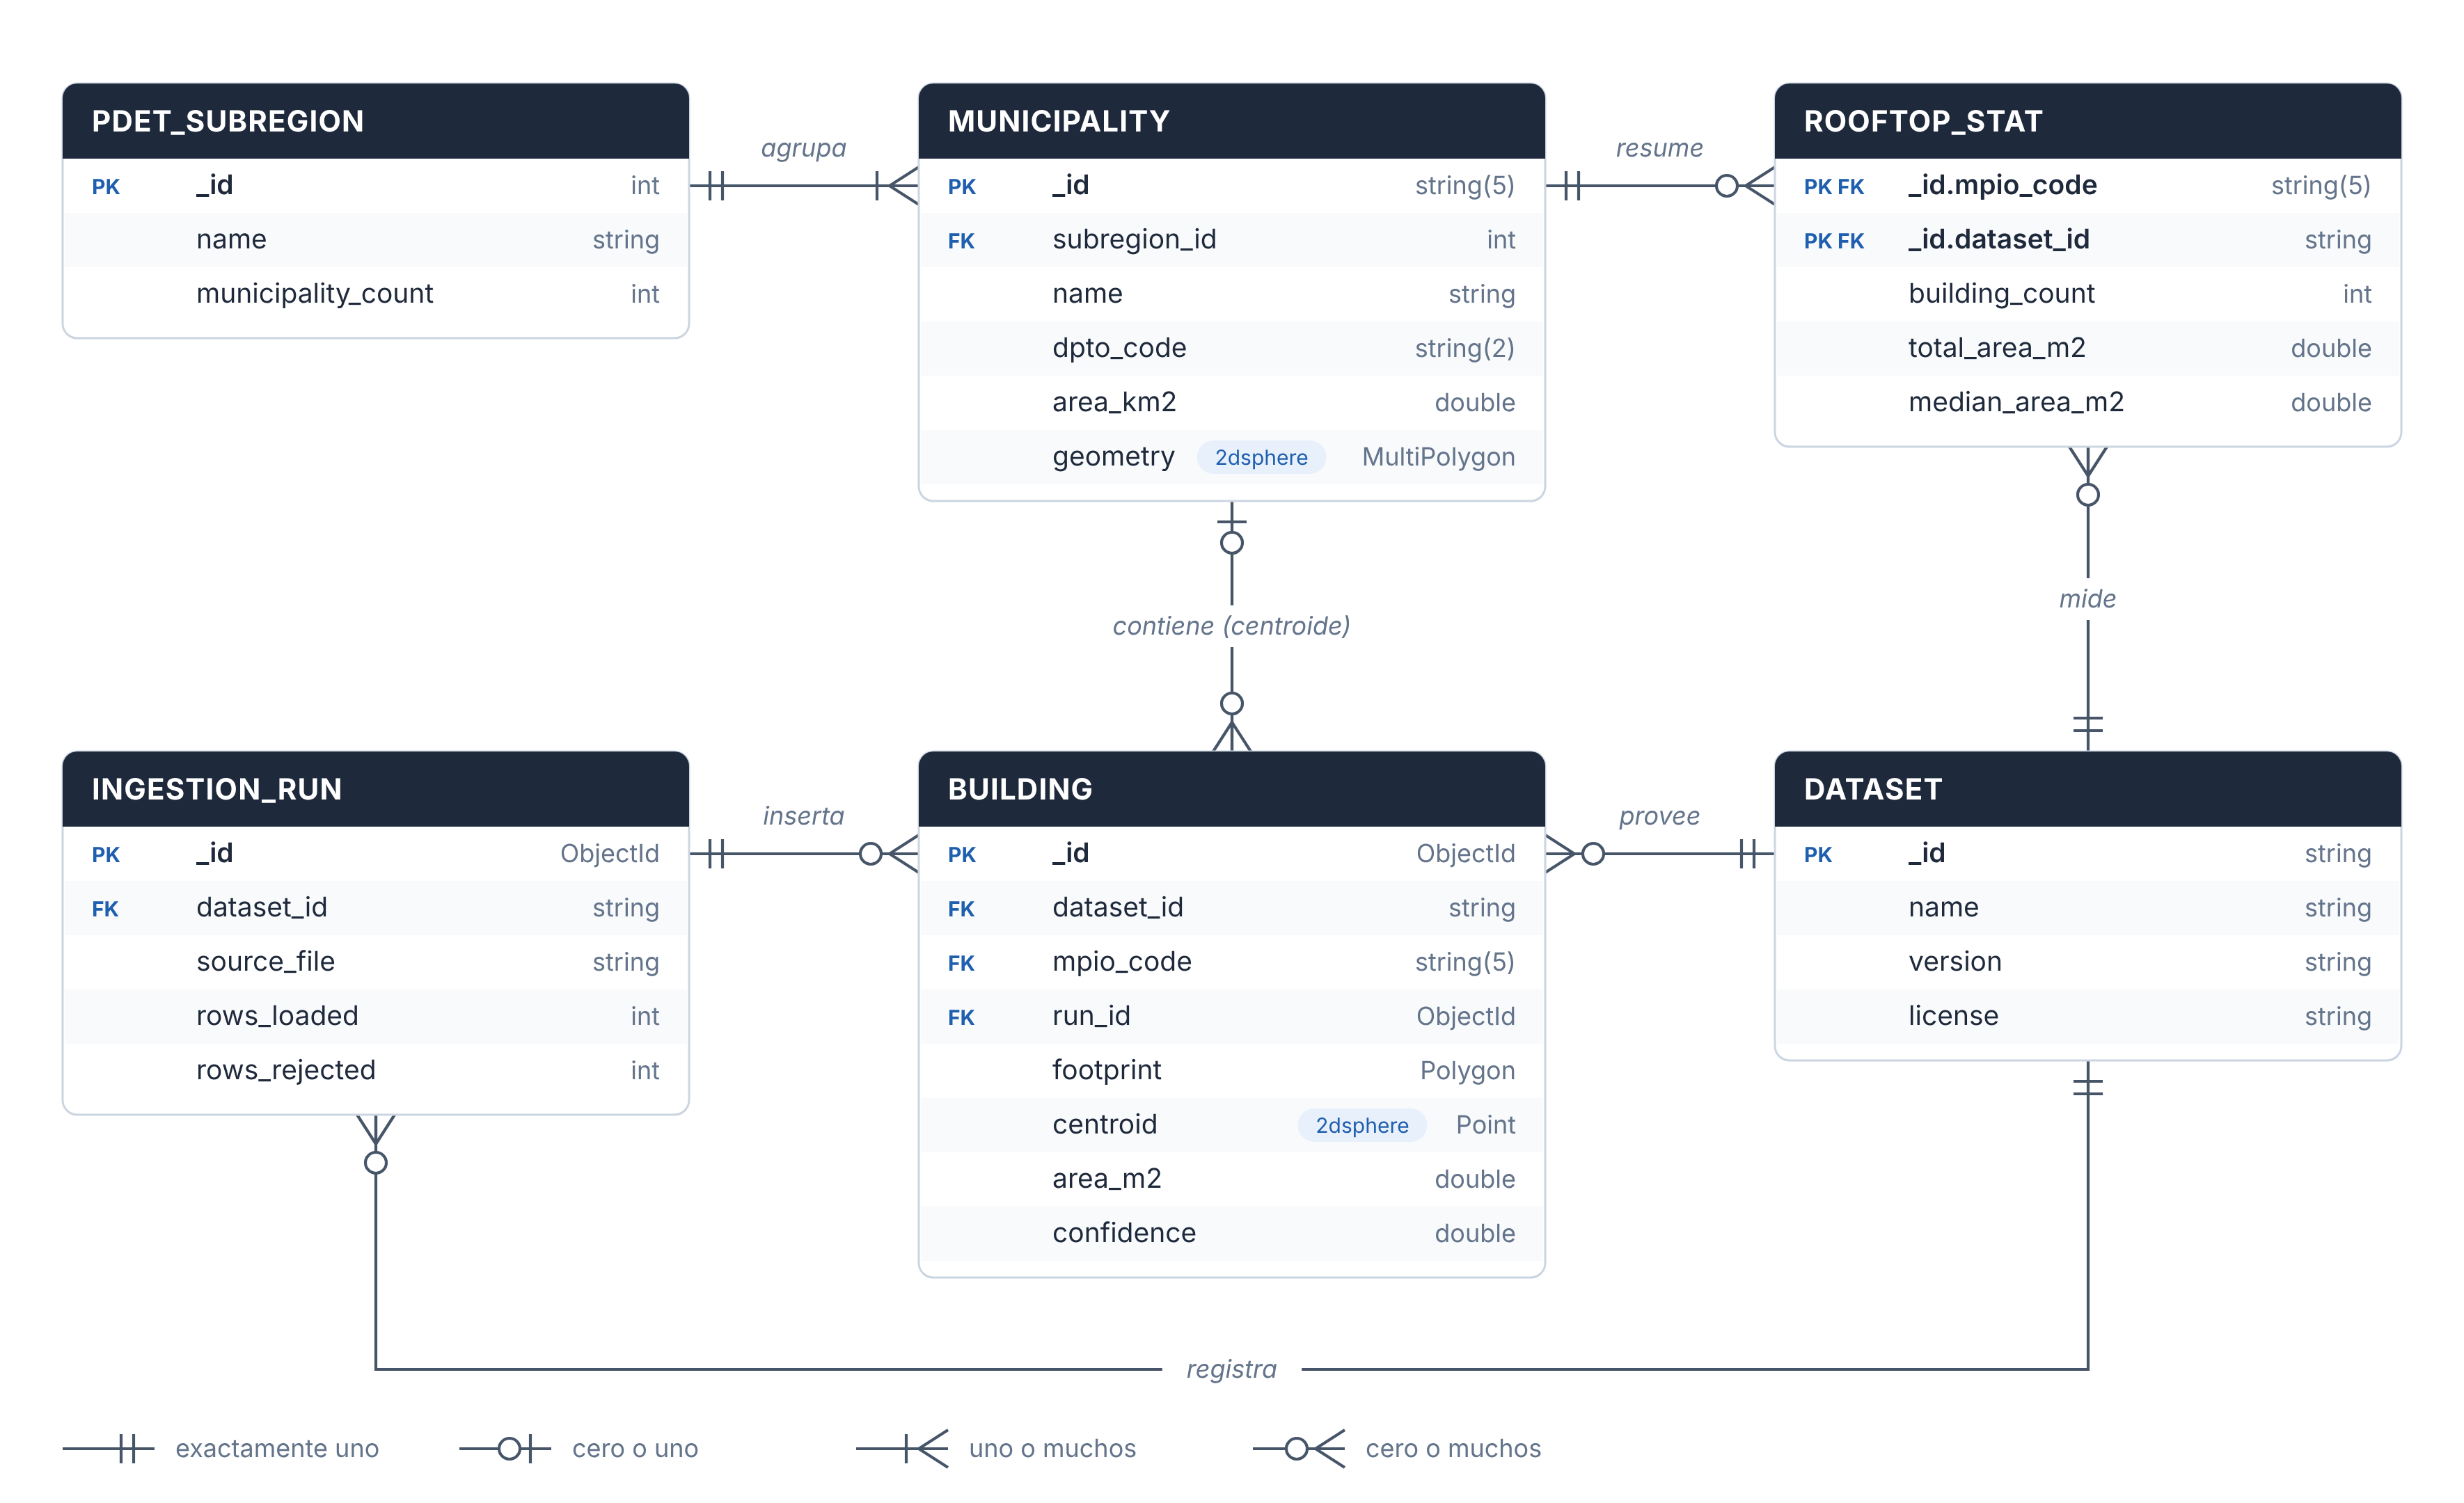
\includegraphics[width=0.95\textwidth]{diagrama_er.png}
\caption{Diagrama E-R en notación pata de gallo: 6 entidades y 7 relaciones. La relación MUNICIPALITY--BUILDING es espacial y opcional: \f{mpio\_code} se llena con \f{\$geoWithin} en la fase 3 y queda en \f{null} si el centroide cae fuera de los municipios PDET. Se genera con \f{docs/delivery1/er/build\_er.py}; versión Mermaid en \f{docs/delivery1/diagrama\_er.md}.}
\end{figure}

\begin{table}[H]
\centering\small
\caption{Del modelo E-R a documentos de MongoDB. Las 7 relaciones se agrupan en 5 patrones.}
\begin{tabularx}{\textwidth}{@{}>{\raggedright\arraybackslash}p{4.4cm} >{\raggedright\arraybackslash}p{4.3cm} L@{}}
\toprule
Relación & Patrón & Motivo \\
\midrule
SUBREGION $\rightarrow$ MUNICIPALITY & Referencia \f{subregion\_id} + copia de \f{subregion\_name} & Los reportes agrupan por subregión sin \f{\$lookup} \\
MUNICIPALITY $\rightarrow$ BUILDING & Referencia \f{mpio\_code} en cada edificación & Millones de edificaciones no caben embebidas (16 MB por documento) \\
DATASET $\rightarrow$ BUILDING & Referencia \f{dataset\_id} & Las dos fuentes en una colección: la misma consulta las compara \\
MUNICIPALITY + DATASET $\rightarrow$ ROOFTOP\_STAT & \f{\_id} compuesto \f{\{mpio\_code, dataset\_id\}} & Un resultado por municipio y fuente; recalcular sobrescribe \\
DATASET $\rightarrow$ INGESTION\_RUN $\rightarrow$ BUILDING & Referencias \f{dataset\_id}, \f{run\_id} & Cada edificación se rastrea hasta el archivo y la carga que la insertó \\
\bottomrule
\end{tabularx}
\end{table}

\section{Diccionario de datos}

Los nombres de colecciones y campos quedan en inglés, igual que en el código. \textbf{*} indica campo obligatorio, exigido por el validador \f{\$jsonSchema}.

\newcommand{\dict}[2]{%
\par\smallskip\textbf{\f{#1}}\par\nopagebreak
{\small\begin{tabularx}{\textwidth}{@{}p{3.3cm} p{3.4cm} L@{}}
\toprule Campo & Tipo & Descripción \\ \midrule #2 \bottomrule
\end{tabularx}}\par}

\dict{pdet\_subregions}{%
\f{\_id}* & int (1--16) & Columna \f{id} de \f{MunicipiosPDET.xlsx} \\
\f{name}* & string & Nombre de la subregión, p.\,ej. ``Alto Patía y Norte del Cauca'' \\
\f{municipality\_count}* & int & Municipios PDET de la subregión \\}

\dict{municipalities}{%
\f{\_id}* & string (5 dígitos) & Código DIVIPOLA (\f{MPIO\_CDPMP}), p.\,ej. \f{19050} \\
\f{name}* & string & Nombre (\f{MPIO\_CNMBR}) \\
\f{dpto\_code}*, \f{dpto\_name}* & string (2 dígitos), string & Departamento (\f{DPTO\_CCDGO}) \\
\f{subregion\_id}*, \f{subregion\_name}* & int, string & Referencia a \f{pdet\_subregions} y copia del nombre \\
\f{area\_km2}* & double & Área oficial (\f{MPIO\_NAREA}) \\
\f{geometry}* & GeoJSON Polygon / MultiPolygon & Límite en WGS84; índice \f{2dsphere} \\
\f{source}*, \f{loaded\_at}* & object, date & \f{\{dataset: "MGN", version: "2025", file\}} y fecha de carga \\}

\dict{datasets}{%
\f{\_id}* & string & \f{ms}, \f{google} o \f{mgn} (límites DANE) \\
\f{name}*, \f{version}*, \f{license}* & string & Nombre, versión (p.\,ej. \f{v3}) y licencia \\
\f{url}*, \f{accessed\_at}* & string, date & Fuente de descarga y fecha de acceso \\}

\dict{buildings}{%
\f{\_id}* & ObjectId & Generado por MongoDB \\
\f{dataset\_id}* & string & Referencia a \f{datasets} \\
\f{source\_ref} & string & ID original (Google: \f{full\_plus\_code}; Microsoft: archivo + fila) \\
\f{footprint}* & GeoJSON Polygon & Contorno del techo en WGS84 \\
\f{centroid}* & GeoJSON Point & Centroide; índice \f{2dsphere}; base de la asignación \\
\f{area\_m2}* & double & Área geodésica (\f{pyproj.Geod}) \\
\f{area\_src\_m2} & double & Área reportada por Google, para validar \\
\f{confidence} & double (0--1) & Confianza de la detección; \f{null} si no viene \\
\f{height\_m} & double & Altura de Microsoft; \f{null} si es $-1$ \\
\f{mpio\_code} & string (5 dígitos) & Referencia a \f{municipalities}; se llena en la fase 3 \\
\f{run\_id}* & ObjectId & Referencia a \f{ingestion\_runs} \\}

\dict{rooftop\_stats}{%
\f{\_id}* & object & \f{\{mpio\_code, dataset\_id\}} \\
\f{building\_count}* & int & Edificaciones con centroide en el municipio, tras filtros \\
\f{total\_area\_m2}*, \f{mean\_area\_m2}*, \f{median\_area\_m2}* & double & Suma, promedio y mediana de \f{area\_m2} \\
\f{filters}*, \f{computed\_at}* & object, date & \f{\{min\_area\_m2, min\_confidence\}} aplicados y fecha del cálculo \\}

\dict{ingestion\_runs}{%
\f{\_id}* & ObjectId & Generado por MongoDB \\
\f{dataset\_id}*, \f{source\_file}* & string & Referencia a \f{datasets} y archivo o partición cargada \\
\f{rows\_read}*, \f{rows\_loaded}*, \f{rows\_rejected}* & int & Contadores de la carga \\
\f{started\_at}*, \f{finished\_at}* & date & Inicio y fin de la carga \\
\f{notes} & string & Errores o advertencias \\}

\section{Índices y validación del esquema}\label{sec:indices}

\begin{table}[H]
\centering\small
\caption{Índices. Indexar el centroide (un punto) y no el polígono hace el índice más pequeño y la prueba de punto en polígono más barata sobre millones de documentos.}
\begin{tabularx}{\textwidth}{@{}l l l L@{}}
\toprule
Colección & Clave & Tipo & Uso \\
\midrule
\f{municipalities} & \f{geometry} & 2dsphere & Consultas espaciales contra los límites \\
\f{municipalities} & \f{subregion\_id} & B-tree & Agrupar por subregión \\
\f{buildings} & \f{centroid} & 2dsphere & Asignación con \f{\$geoWithin} (consulta principal) \\
\f{buildings} & \f{\{dataset\_id, mpio\_code\}} & Compuesto & Agregar por fuente y municipio \\
\f{ingestion\_runs} & \f{dataset\_id} & B-tree & Auditar cargas por fuente \\
\bottomrule
\end{tabularx}
\end{table}

\f{scripts/00\_init\_db.py} crea las seis colecciones con validadores \f{\$jsonSchema} (campos obligatorios y tipos de la sección anterior) y los índices de la tabla. Los índices de \f{buildings} se crean con \f{-{}-building-indexes} después de la carga masiva, para no frenar las inserciones. Lo probamos contra MongoDB 7.0:

\begin{itemize}
  \item Se crean las 6 colecciones y los 5 índices (los 2 de \f{buildings} con \f{-{}-building-indexes}); correrlo dos veces no cambia nada.
  \item Un municipio con código \f{5031} (4 dígitos) es rechazado por el validador.
  \item \f{\$geoWithin} sobre \f{buildings.centroid} usa el índice \f{centroid\_2dsphere} según \f{explain()}.
\end{itemize}

\section{Riesgos y mitigaciones}

\begin{table}[H]
\centering\small
\begin{tabularx}{\textwidth}{@{}>{\raggedright\arraybackslash}p{6.2cm} L@{}}
\toprule
Riesgo & Mitigación \\
\midrule
Los archivos de edificaciones cubren todo el país y no caben en memoria & Descargar solo particiones que tocan los rectángulos PDET; leer por bloques; filtrar antes de insertar \\
Polígonos inválidos: el índice \f{2dsphere} de \f{municipalities} los rechaza, y una huella inválida da área y centroide errados & \f{make\_valid} antes de insertar; \f{rows\_rejected} y \f{notes} en \f{ingestion\_runs} \\
Los nombres de la lista PDET no coinciden con los del MGN & Cruzar por código DIVIPOLA \\
El MultiPolygon de un municipio supera 16 MB & Medir el tamaño al cargar; simplificar con tolerancia fija solo si hace falta y documentarlo \\
Las dos fuentes dan conteos distintos para un municipio & Reportar ambas cifras y su diferencia; no promediarlas \\
\bottomrule
\end{tabularx}
\end{table}

\section{Repositorio y responsables}

\begin{table}[H]
\centering\small
\begin{tabularx}{\textwidth}{@{}l L L@{}}
\toprule
Integrante & Aporte a la Entrega 1 & Archivos \\
\midrule
Miguel Duarte & Estructura del repositorio, configuración, diagrama E-R y primera versión del documento & \f{README.md}, \f{config.yaml}, \f{docker-compose.yml}, \f{diagrama\_er.png} \\
Derek Sarmiento & Esquema implementado (validadores e índices), diagrama E-R final y este documento en \LaTeX & \f{scripts/00\_init\_db.py}, \f{docs/delivery1/er/build\_er.py}, \f{docs/delivery1/entrega1.tex} \\
José Medina & Verificación de la lista PDET (170 municipios, 16 subregiones) & \f{scripts/00\_check\_pdet\_list.py} \\
Sebastián Sánchez Vásquez & Verificación del entorno y credenciales fuera del código & \f{scripts/00\_check\_environment.py}, \f{.env.example} \\
Samuel Emperador & Diagrama E-R editable en Mermaid & \f{docs/delivery1/diagrama\_er.md} \\
\bottomrule
\end{tabularx}
\end{table}

Los datos crudos van en \f{data/} (ignorado por git) y los resultados en \f{outputs/}. El \f{README.md} indica el orden de ejecución.

\end{document}
